\chapter{Conclusioni}
\section{Risultati}
Il circuito stampato realizzato \`e funzionante, come il protototipo iniziale
su piastra sperimentale, malgrado gli errori rilevati durante la messa in
servizio.

% \begin{figure}[H] \centering
%     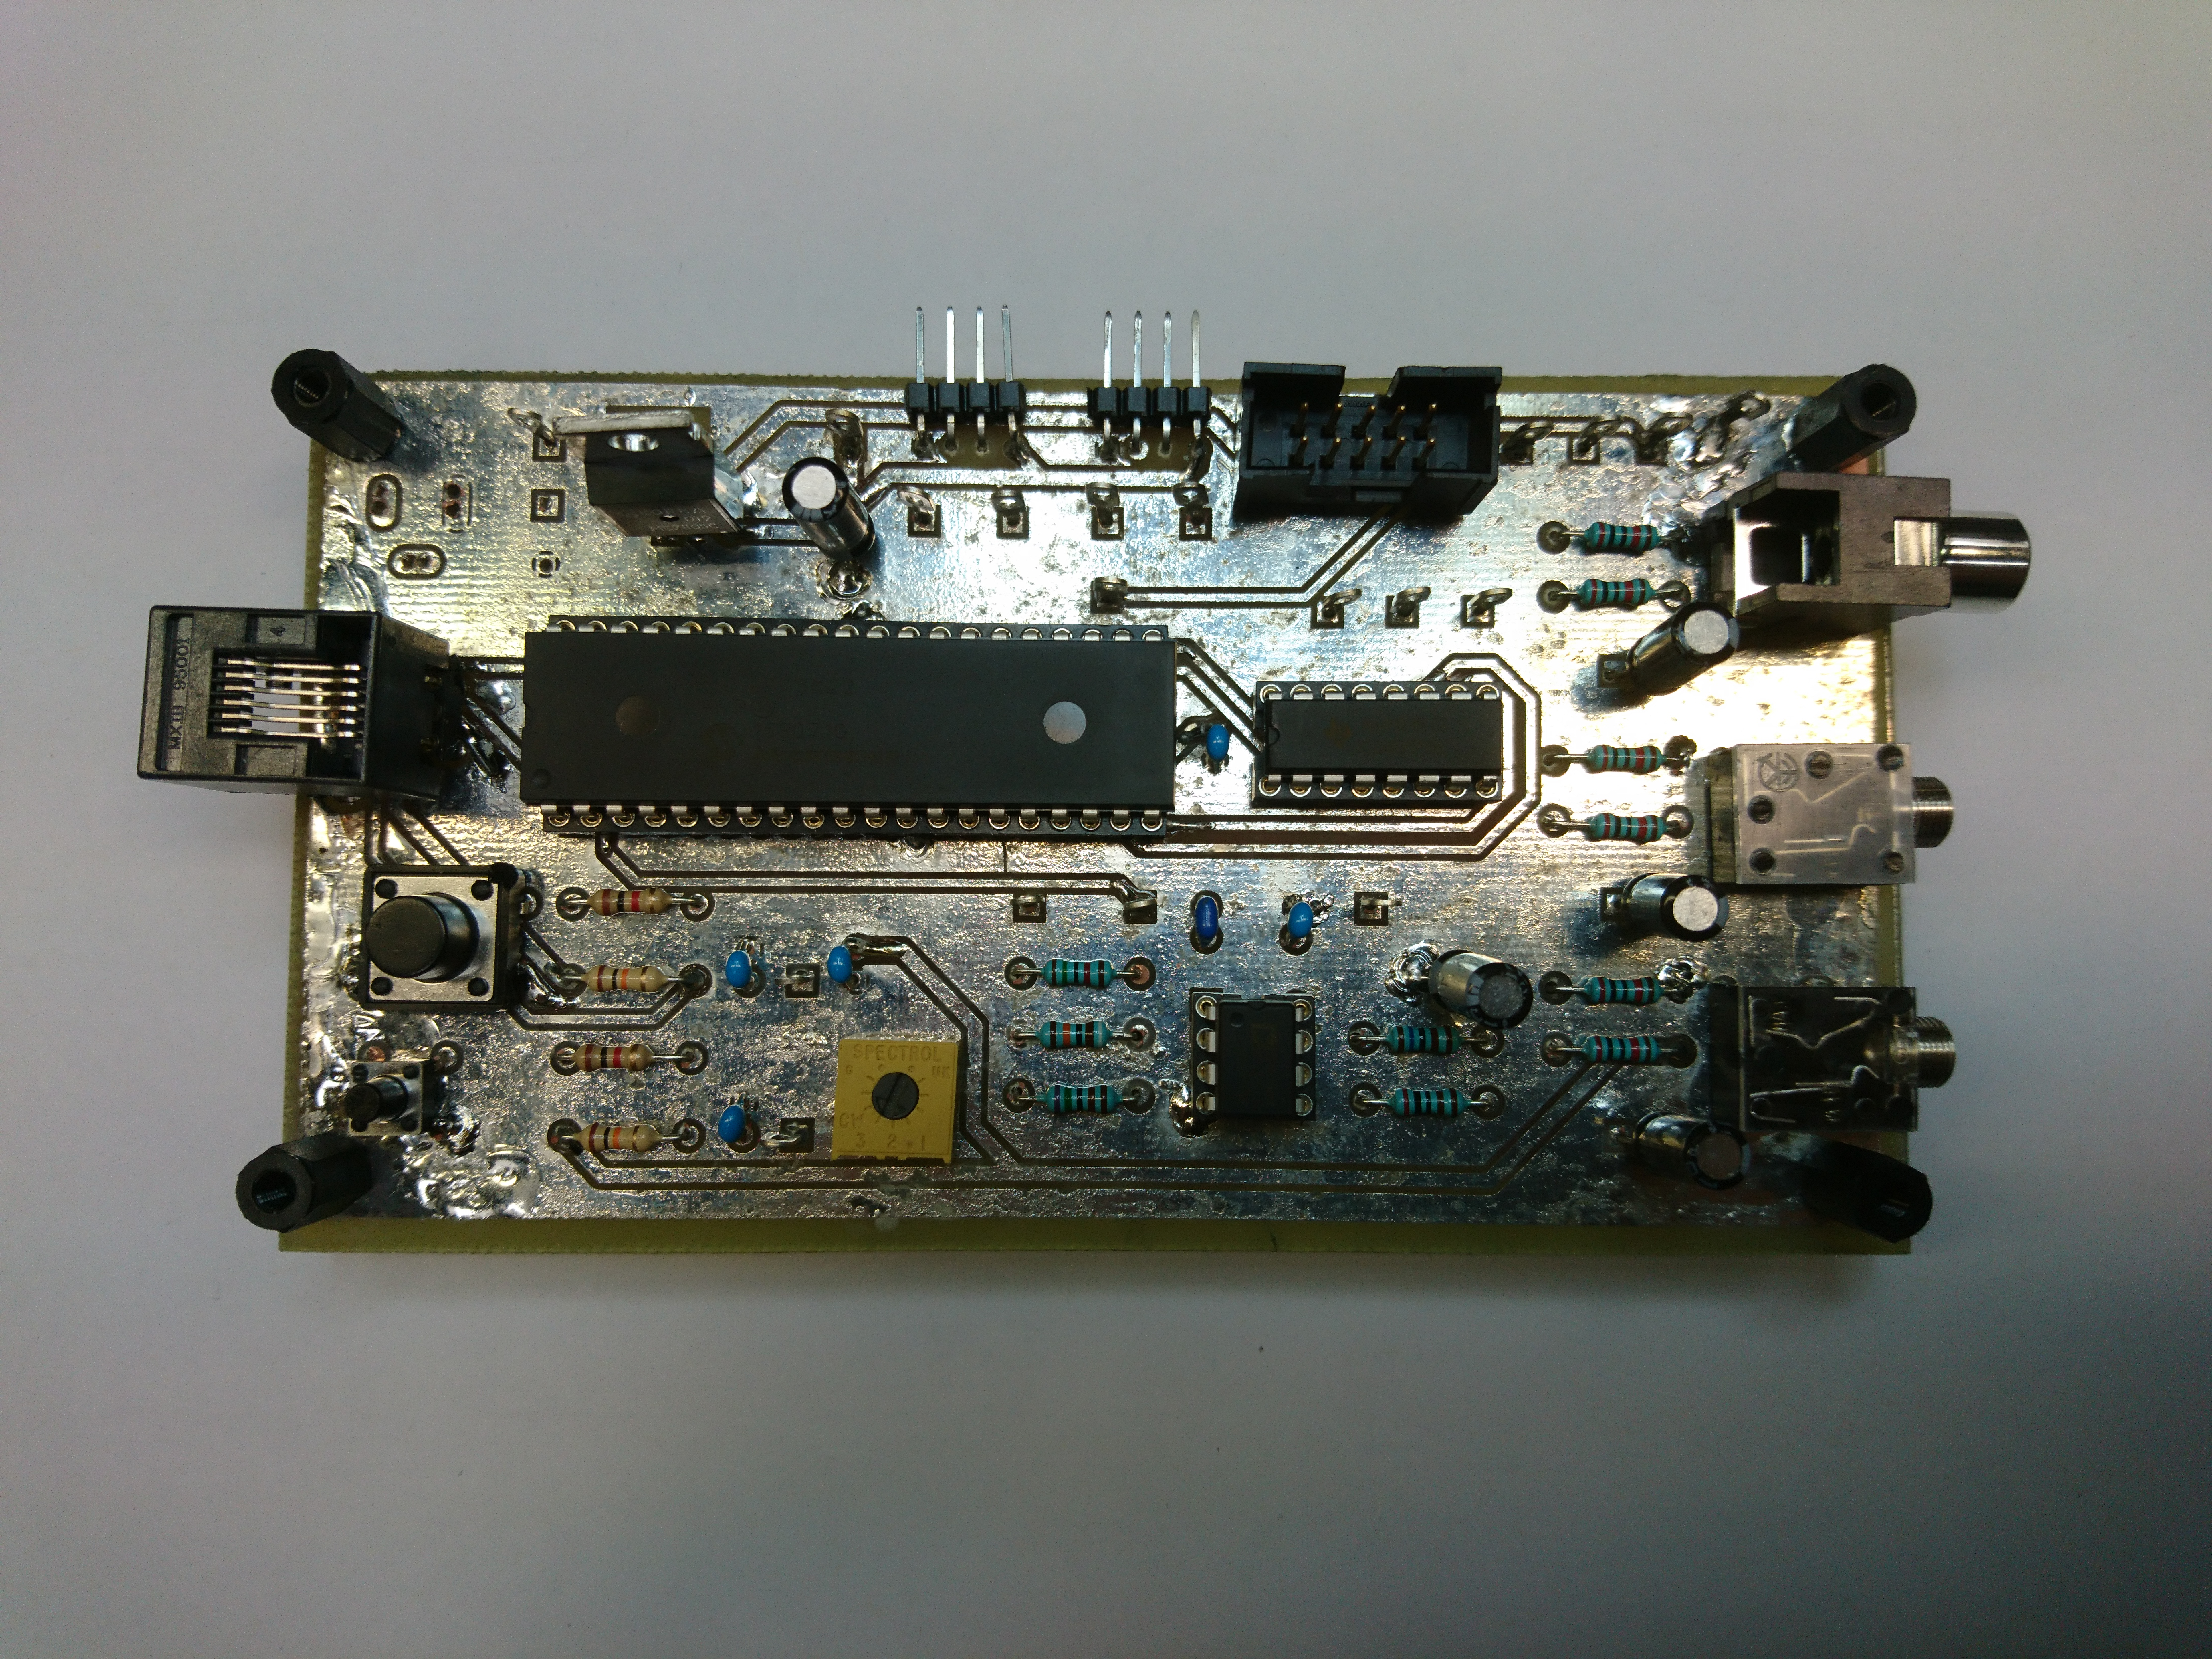
\includegraphics[height=7cm]{figures/photos/pcb-1}
% \end{figure}

\subsection{Esempi di misurazioni}
I dati illustrati nella figura \ref{fig:measurements} sono esportati dal
programma desktop.
\begin{figure}[H] \centering
    \begin{tikzpicture}
        \begin{axis}[
            width = \textwidth,
            height = .4\textwidth,
            axis x line = center,
            axis y line = center,
            xlabel = {\(f\)},
            xlabel style = {right},
            ylabel = {\(A\)},
            ylabel style = {above},
            grid=both,
            grid style = dotted,
            % axis equal,
            % xticklabels = \empty,
            extra x ticks = {-10,-9,...,10},
            extra x tick labels= \empty,
            extra y ticks = {-10,-9,...,10},
            extra y tick labels= \empty,
        ]
            \addplot [smooth, red, mark size=1] table [col sep=comma] {res/data/fft-sine-wave.csv};
            \addplot [smooth, blue, mark size=1] table [col sep=comma] {res/data/fft-square-wave-lf.csv};
        \end{axis}
    \end{tikzpicture}
    \caption{
        Spettro di un'onda sinusoidale (rosso) e di un segnale quadrato (blu)
        \label{fig:measurements}
    }
\end{figure}

\section{Problemi riscontrati}
\subsection{Errore nella scelta dell'opamp}
\label{sec:err-opamp}

Durante la fase di test, dopo l'assemblaggio, si \`e notato che
l'amplificatore operazionale AD826 non \`e un opamp rail to rail, come l'AD820
utilizzato durante la fase di sviluppo su piastra sperimentale.  Ci\`o limita
l'escursione del segnale amplificato di quasi 1\,V, riducendo la precisione
del campionamento.

Fortunatamente il pinout DIP8 degli operazionali dual package \`e standard,
perci\`o non vi sono eccessive difficolt\`a nella sostituzione del componente.
Purtroppo per\`o non sar\`a possibile acquistare in tempo un opamp
sostitutivo. Un possibile sostituto, utilizzato nella seconda revisione dello
schema, potrebbe essere l'operazionale MCP6292 (in alternativa: MCP6002, TI
OPA2340, ICL7621DCPAZ).

\subsection{Errore nel dimensionamento del filtro attivo}
\label{sec:err-filter}

Durante la fase di test \`e stato inoltre rilevato che il filtro attivo (vedi
figura \ref{fig:filter-ampl-v1}) di anti-alias aveva un amplificazione non
unitaria, dunque incorretta.  La tensione di offset di 2.5\,V veniva
amplificata ed in molti punti l'operazionale entrava in saturazione.  Ci\`o
era causato dal valore incorretto di \(R_{11}\) poich\`e l'amplificazione,
data dalla relazione sottostante, era  di 2.
\[
    A_v = 1+R_{12}/R_{11} = 1+15\,\text{k}\Omega/15\,\text{k}\Omega = 2
\]

Un valore sostitutivo per il resistore \(R_{11}\) \`e
\(\geq 750\,\text{k}\Omega\), in modo da ottenere un amplificazione quasi
unitaria, con un errore di \(+0.02\), che corrisponde ad un incremento di
50\,mV della tensione di offset di 2.5\,V. Valori di ordini di grandezza
maggiori sono preferibili, infatti dopo aver rilevato il guasto a \(R_{11}\)
\`e stato assegnato un valore di \(910\,\text{k}\Omega\).
\[
    A_v = 1+R_{12}/R_{11} = 1+15\,\text{k}\Omega/910\,\text{k}\Omega \approx 1.016
\]

Cos\`i facendo per\`o \`e stata modificata la frequenza di taglio del filtro.
Perci\`o si \`e concluso che il circuito scelto non \`e utilizzabile e nella
seconda revisione la configurazione \`e stata sostituita da una cella RC con
un amplificatore non invertente.

\subsection{Sincronizzazione dei threads}
\label{sec:err-sync}
Durante lo sviluppo del software desktop \`e stato riscontrato un unico
problema riguardante la sincronizzazione dei threads. La risorsa
\texttt{serial::Serial MainWindow::\_serial}  come implica il nome \`e
instanziata nella classe \texttt{MainWindow}, ma essa \`e gestita anche dalla
classe \texttt{SerialWorker} siccome \`e suo compito leggere i dati.

Perci\`o la risorsa deve essere protetta da un \texttt{QMutex} e la sua
\emph{lifetime} (ciclo di vita) deve essere gestita tenendo in considerazione
il thread parallelo.  Il bug era causato da una chiusura della risorsa seriale
mentre il thread era ancora attivo.  Chiudendo la risorsa mentre il thread del
\texttt{SerialWorker} \`e attivo, al tentativo di lettura seguente il metodo
\texttt{serial::Serial::read()} causa una \texttt{serial::IOException} che fa
crashare il programma.

La ragione per cui il thread non veniva fermato, era l'utilizzo incorretto
dell'API dei \texttt{QThread}. Per chiudere correttamente un thread secondo il
framework di Qt si richiede un interruzione con
\texttt{QThread::requestInterruption()}. Invece nel codice veniva utilizzato
\texttt{QThread::quit()}, che se non in condizioni particolari non chiude il
processo parallelo.

Il diff  sottostante mostra il commit in cui il problema viene risolto.
\lstinputlisting[language=diff]{res/serialworker-crash-fix.diff}

\section{Possibili miglioramenti e sviluppi futuri}
\subsection{Filtro}
Il circuito di filtraggio del rumore di alta frequenza potrebbe essere
sostituito con un filtro di secondo o di terzo ordine per migliorarne le
prestazioni.

\subsection{Circuito di selezione dell'entrata}
Il multiplexer utilizzato per l'entrata ha un valore d'impedenza non
particolarmente eccezionale, per migliorare le prestazioni si dovrebbe
scegliere un multiplexer differente.

\subsection{Supporto per MacOS}
Il software (al computer) dell'analisi spettrale attualmente non utilizza
dipendenze che richiedono una piattaforma particolare. Portare il software per
MacOS non dovrebbe essere difficile.


\subsection{Supporto per altri formati di dati}
Il software al computer attualmente supporta unicamente il formato CSV (Comma
Separated Values) per l'esportazione dei dati. Sarebbe opportuto aggiungere il
supporto di altri formati come DAT (Data), TSV (Tab Separated Values) e ODS
(Open Document format for Spreadsheet).

\section{Commento}
Personalmente ho trovato il progetto molto interessante e coinvolgente.
Malgrado la complessit\`a dell'argomento trattato, grazie al supporto di
docenti ed amici, sono riuscito ad avere una comprensione tutto sommato
abbastanza completa del funzionamento del principio matematico dell'analisi
spettrale.

\section{Ringraziamenti}
Vorrei ringraziare Eduardo Cima: professore di elettrotecnica alla SAM e
Raffaele Ancarola: studente di fisica del primo anno al Politecnico Federale
di Losanna (EPFL), per il grande supporto attraverso spiegazioni e chiarimenti
degli strumenti matematici della trasformata di Fourier; ed infine vorrei
ringraziare anche il professor Emidio Planamente per l'aiuto a risolvere il
bug di sincronizzazione (\ref{sec:err-sync}).


\section{Certificazione}
Il sottoscritto dichiara di aver redatto e prodotto individualmente il lavoro
di produzione.
\begin{flushright}
\begin{tabular}{ r p{5cm} p{1cm} r p{5cm}}
    Data: & \hrulefill && Firma: & \hrulefill \\
    &&&& Naoki Pross \\
\end{tabular}
\end{flushright}
